% Options for packages loaded elsewhere
\PassOptionsToPackage{unicode}{hyperref}
\PassOptionsToPackage{hyphens}{url}
\PassOptionsToPackage{dvipsnames,svgnames*,x11names*}{xcolor}
%
\documentclass[
]{article}
\usepackage{amsmath,amssymb}
\usepackage{lmodern}
\usepackage{ifxetex,ifluatex}
\ifnum 0\ifxetex 1\fi\ifluatex 1\fi=0 % if pdftex
  \usepackage[T1]{fontenc}
  \usepackage[utf8]{inputenc}
  \usepackage{textcomp} % provide euro and other symbols
\else % if luatex or xetex
  \usepackage{unicode-math}
  \defaultfontfeatures{Scale=MatchLowercase}
  \defaultfontfeatures[\rmfamily]{Ligatures=TeX,Scale=1}
\fi
% Use upquote if available, for straight quotes in verbatim environments
\IfFileExists{upquote.sty}{\usepackage{upquote}}{}
\IfFileExists{microtype.sty}{% use microtype if available
  \usepackage[]{microtype}
  \UseMicrotypeSet[protrusion]{basicmath} % disable protrusion for tt fonts
}{}
\makeatletter
\@ifundefined{KOMAClassName}{% if non-KOMA class
  \IfFileExists{parskip.sty}{%
    \usepackage{parskip}
  }{% else
    \setlength{\parindent}{0pt}
    \setlength{\parskip}{6pt plus 2pt minus 1pt}}
}{% if KOMA class
  \KOMAoptions{parskip=half}}
\makeatother
\usepackage{xcolor}
\IfFileExists{xurl.sty}{\usepackage{xurl}}{} % add URL line breaks if available
\IfFileExists{bookmark.sty}{\usepackage{bookmark}}{\usepackage{hyperref}}
\hypersetup{
  colorlinks=true,
  linkcolor=Maroon,
  filecolor=Maroon,
  citecolor=Blue,
  urlcolor=blue,
  pdfcreator={LaTeX via pandoc}}
\urlstyle{same} % disable monospaced font for URLs
\usepackage{graphicx}
\makeatletter
\def\maxwidth{\ifdim\Gin@nat@width>\linewidth\linewidth\else\Gin@nat@width\fi}
\def\maxheight{\ifdim\Gin@nat@height>\textheight\textheight\else\Gin@nat@height\fi}
\makeatother
% Scale images if necessary, so that they will not overflow the page
% margins by default, and it is still possible to overwrite the defaults
% using explicit options in \includegraphics[width, height, ...]{}
\setkeys{Gin}{width=\maxwidth,height=\maxheight,keepaspectratio}
% Set default figure placement to htbp
\makeatletter
\def\fps@figure{htbp}
\makeatother
\setlength{\emergencystretch}{3em} % prevent overfull lines
\providecommand{\tightlist}{%
  \setlength{\itemsep}{0pt}\setlength{\parskip}{0pt}}
\setcounter{secnumdepth}{-\maxdimen} % remove section numbering
\ifluatex
  \usepackage{selnolig}  % disable illegal ligatures
\fi

\author{}
\date{}

\begin{document}

\hypertarget{building-an-industry-code-classifier}{%
\section{2. Building an Industry Code
Classifier}\label{building-an-industry-code-classifier}}

In this section we describe the construction of a classification model
that is able to assign companies 4-digit SIC codes based on their
business descriptions. This is used to highlight some of the challenges
associated with categorising companies with single industrial
activities. The steps in this process are:

\begin{enumerate}
\def\labelenumi{\arabic{enumi}.}
\tightlist
\item
  Train a supervised text classification model based on company
  descriptions from Glass AI and SIC codes from Companies House.
\item
  Apply the model to a test set of company descriptions not used to
  build the model.
\end{enumerate}

\hypertarget{methodology}{%
\subsection{1. Methodology}\label{methodology}}

The development of the classifier was treated as a supervised machine
learning problem. In practice, there are no official datasets that
contain company descriptions and their associated SIC codes. Therefore,
we combined two sources of data to create our final training dataset.
These are descriptions of companies obtained from their websites by
Glass AI and the SIC code associated with each company from Companies
House. These two datasets do not have innate fields that allow for
direct joining therefore entries from Companies House were matched to
their likely descriptions using a previously developed fuzzy matching
approach.

For the modelling itself, a transformer based approach has been taken.
Transformers are a state-of-the-art neural network architecture that
have shown to produce improved results on many language based machine
learning tasks and have reduced the resources needed to create
performant models. Importantly for this work, pre-trained models whose
parameters have already been tuned on large volumes of text can be fine
tuned for downstream tasks such as text classification. This can be done
with relatively little data. It is this approach that we use here.

For the SIC code classifier, we fine-tuned an English language
DistilBERT model. An additional classification layer was added to this
neural network and it was trained on over 300,000 company descriptions
and their labels. The model was then applied to 50,000 unseen business
descriptions and the predictions were compared to the ``ground truth''
labels.

\hypertarget{results}{%
\subsection{2. Results}\label{results}}

Evaluating a classification model with 615 possible output classes is
not a trivial task never an easy task as overall accuracy metrics often
do not capture the differences and tradeoffs in precision and recall of
the many classes. Specifically in this task there are additional
complicating factors:

\begin{enumerate}
\def\labelenumi{\arabic{enumi}.}
\tightlist
\item
  The 4-digit SIC code labels in the training data are often not
  appropriate for the business description. It is unclear whether this
  is due to the fuzzy matching resulting in some mismatched data or poor
  labelling on Companies House.
\item
  In some cases it is not possible to determine the purpose of the
  company from the website description provided by Glass AI. This might
  be because the text describes other attributes of the company such as
  its founding story, the description may be very short or the text may
  simply be website metadata.
\item
  The dataset is highly imbalanced. With a large number of classes it is
  already challenging to optimise accuracy for all possible labels and
  this is exacerbated by a heavy class imbalance. Some labels are
  represented tens of thousands of times in the training data, many
  others are present fewer than ten times.
\end{enumerate}

Despite these limitations, there are useful insights that can be be
gained from the outputs of the classifier and its predictions. In
{[}@Fig:predicted\_sic4\_representation\_barh{]} we can see 20 predicted
SIC codes that are overrepresented and 20 codes that are
underrepresented compared to the actual codes associated with companies
in the data. Only 95 of the 615 possible 4-digit SIC codes were produced
by the classifier to label companies, suggesting that while the
classifier believes some codes are very widely applicable, there are
many codes that are challenging for the classifier to identify from
company descriptions.

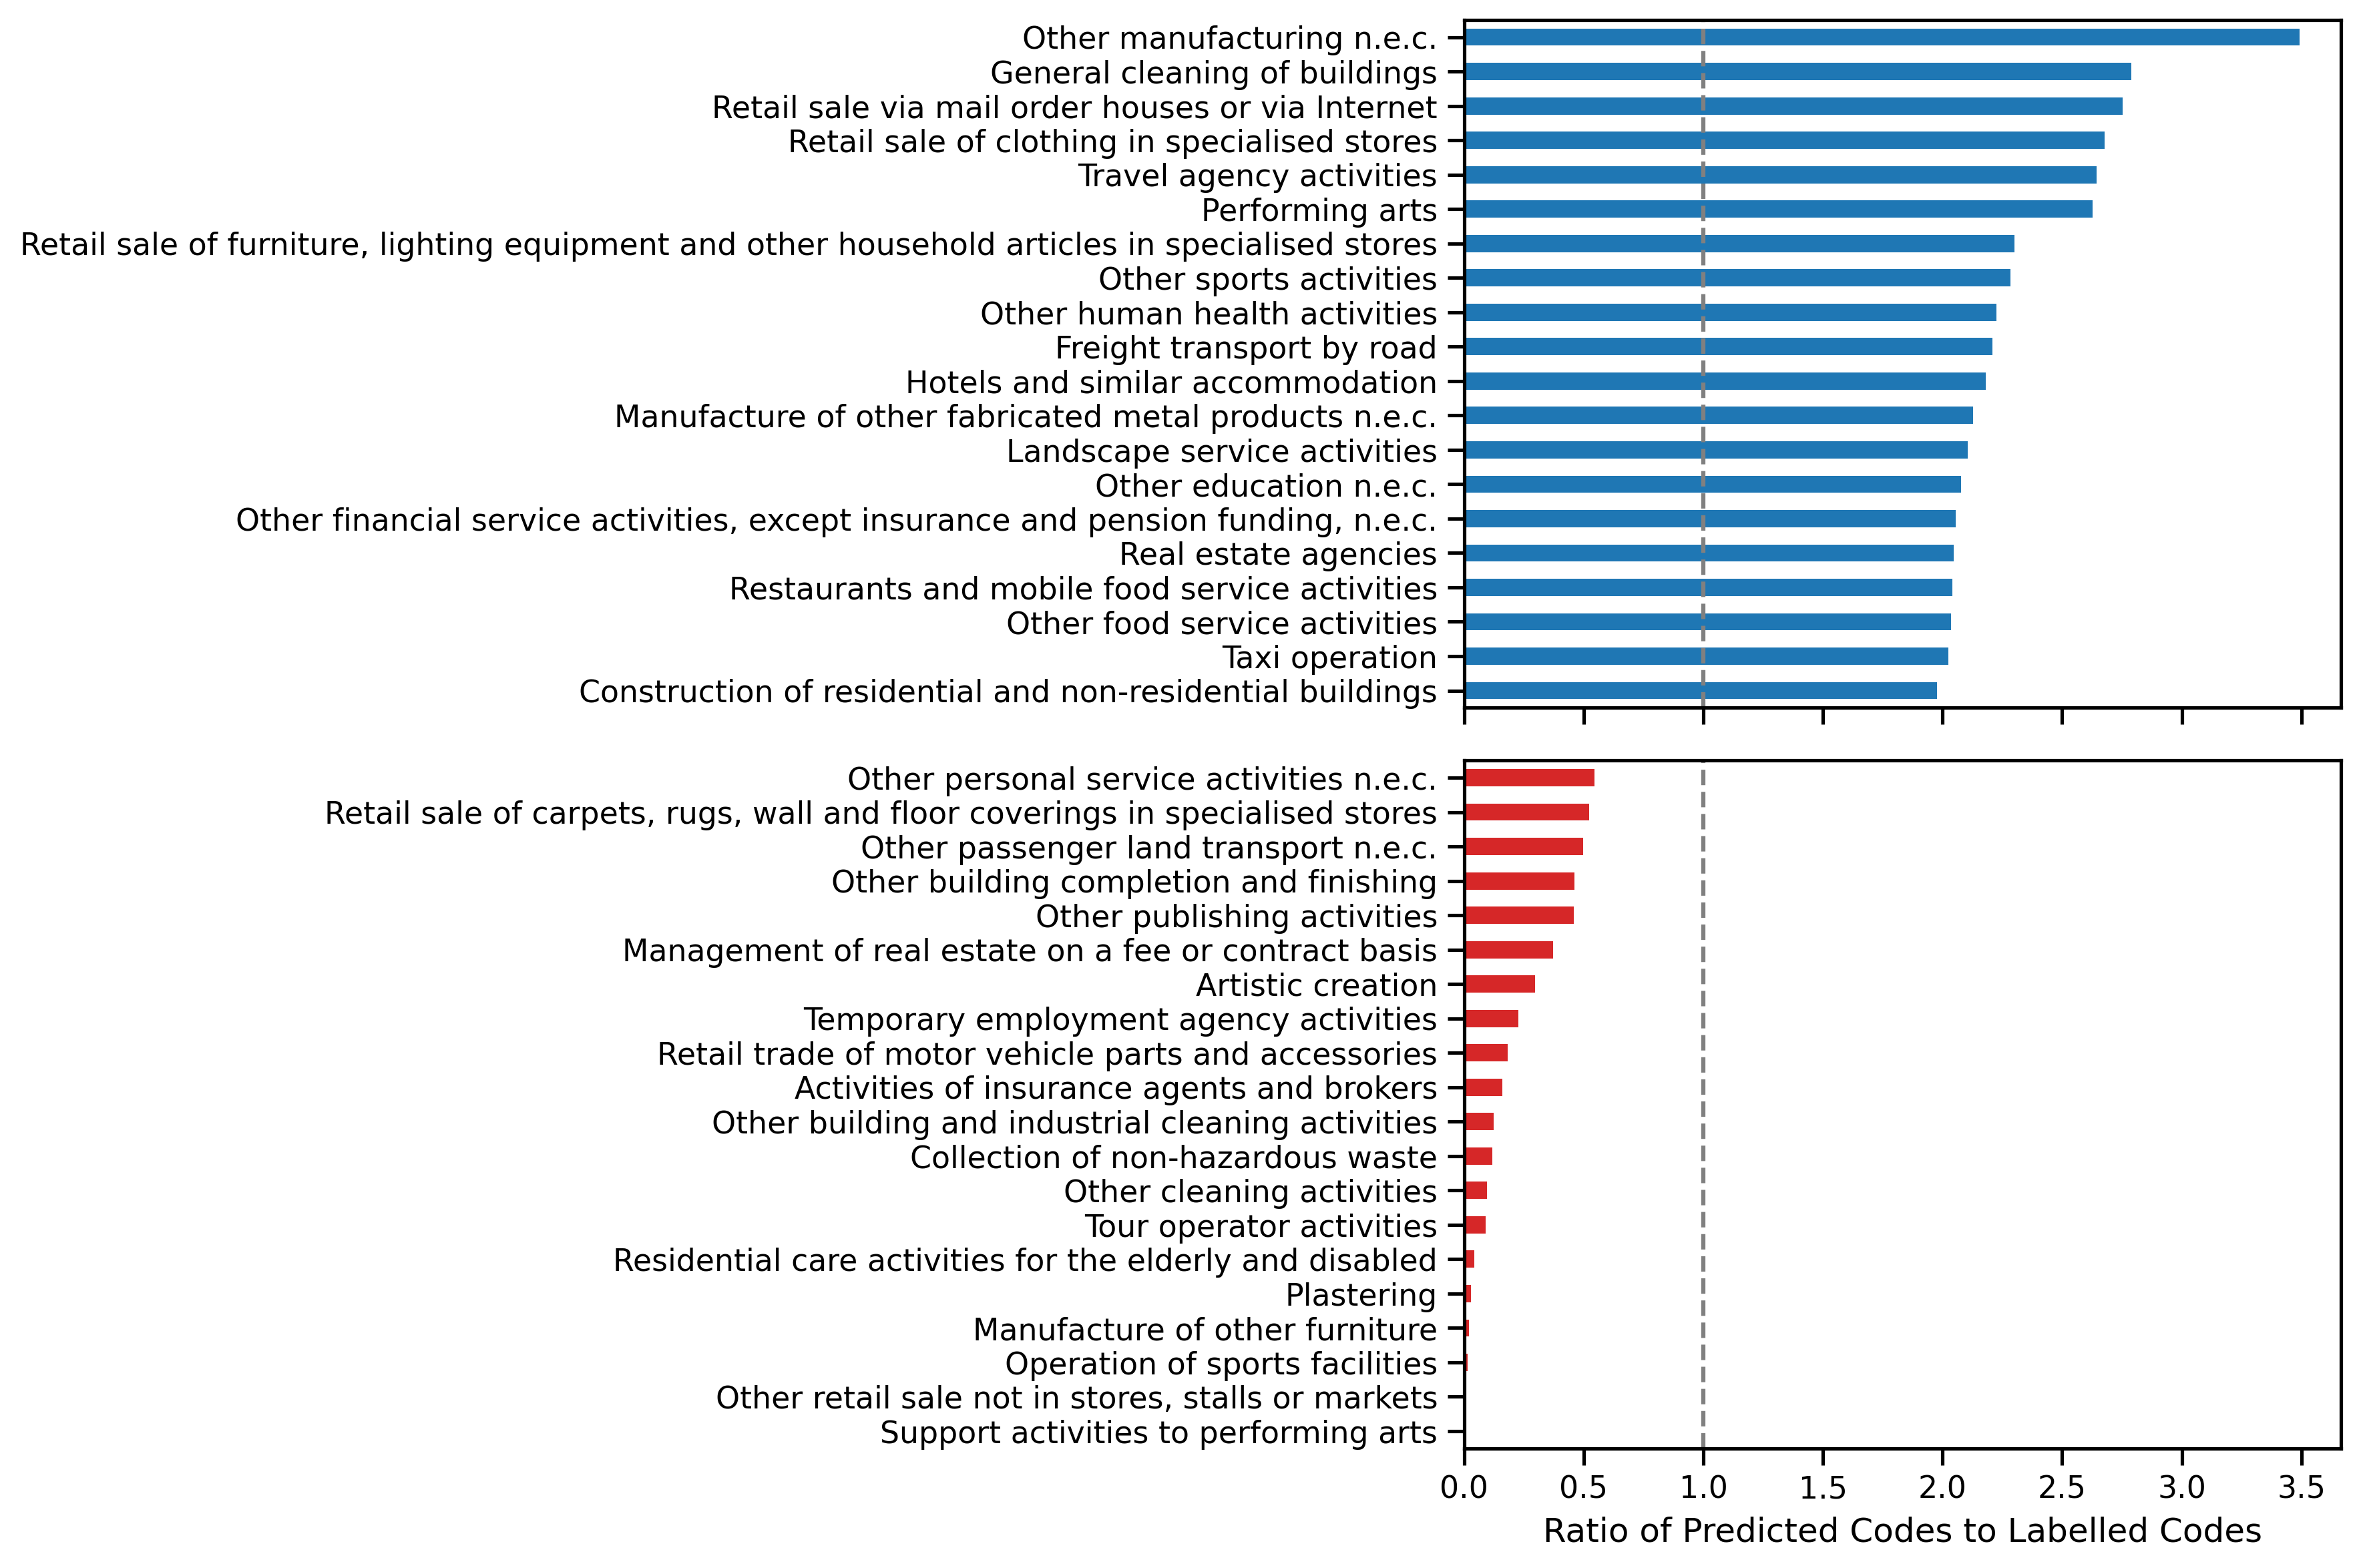
\includegraphics{../../figures/predicted_sic4_representation_barh.png}\{\#fig:
predicted\_sic4\_representation\_barh\}

For each company description, the classifier produces a vector of
4-digit SIC code probabilities. The code with the highest probability is
chosen as the predicted label, however investigating those probabilities
also yields useful insights as to the confidence of the classifier. We
took all of the probabilities for the successfully predicted labels and
aggregated them by 4-digit SIC code to obtain the mean. In this way are
able to see which codes are generally predicted with higher or lower
probabilities. We can see from {[}@Fig:
mean\_sic4\_prediction\_probability\_barh{]} that the codes with higher
prediction probabilities tend to be more widely known whereas the areas
with lower probabilities describe more niche activities.

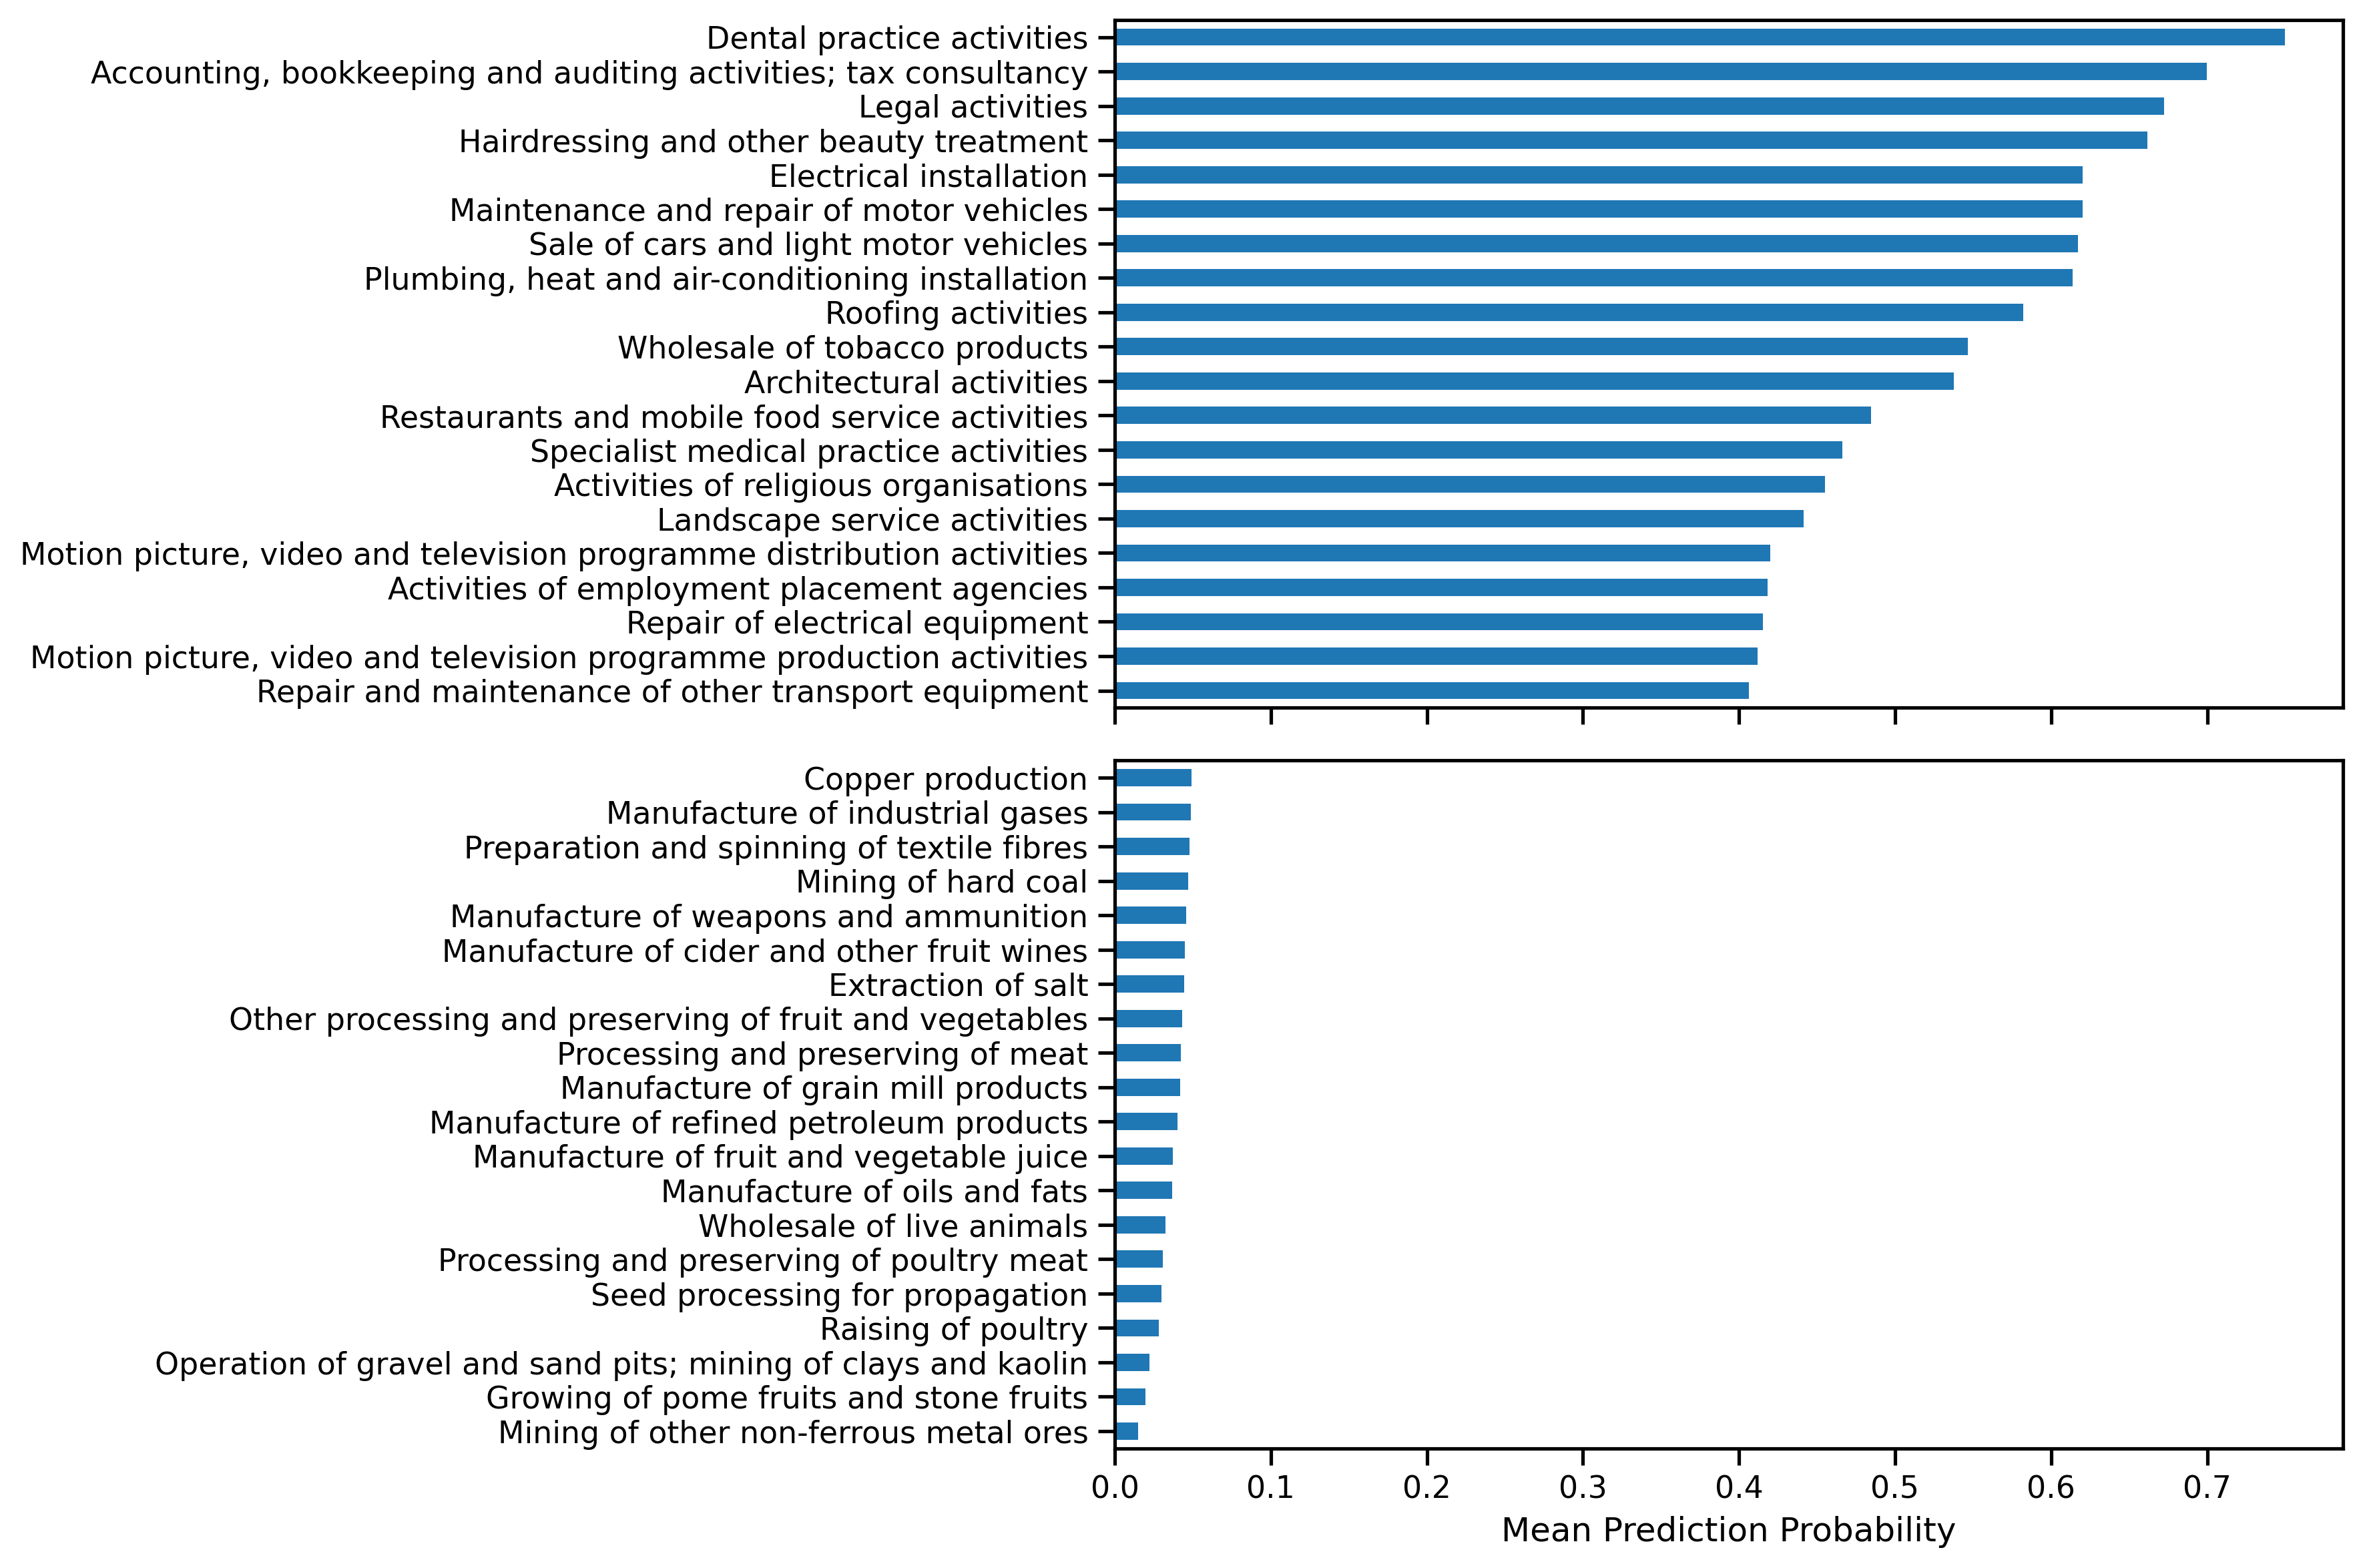
\includegraphics{../../figures/mean_sic4_prediction_probability_barh.png}\{\#fig:
mean\_sic4\_prediction\_probability\_barh\}

While it might be reasonable to suspect that codes are overrepresented
due to their frequency in the training data from which the classifier
has learned, we see that this is not always the case. While there is a
positive correlation between the frequency of 4-digit SIC codes in the
training data and their representation among predicted codes, the
relationship is weak and not linear. There are a number of sectors that
have a high relatively high frequency, but are underrepresented and
vice-versa. The codes highlighted in
\{\#fig:predicted\_sic4\_representation\_vs\_training\_frequency\_scatter\}
show that the extremes consist of quite highly generalised activity
descriptions, suggesting that the model recognises them as catch-all
labels or not sufficiently specific to be used in comparison to other
labels.

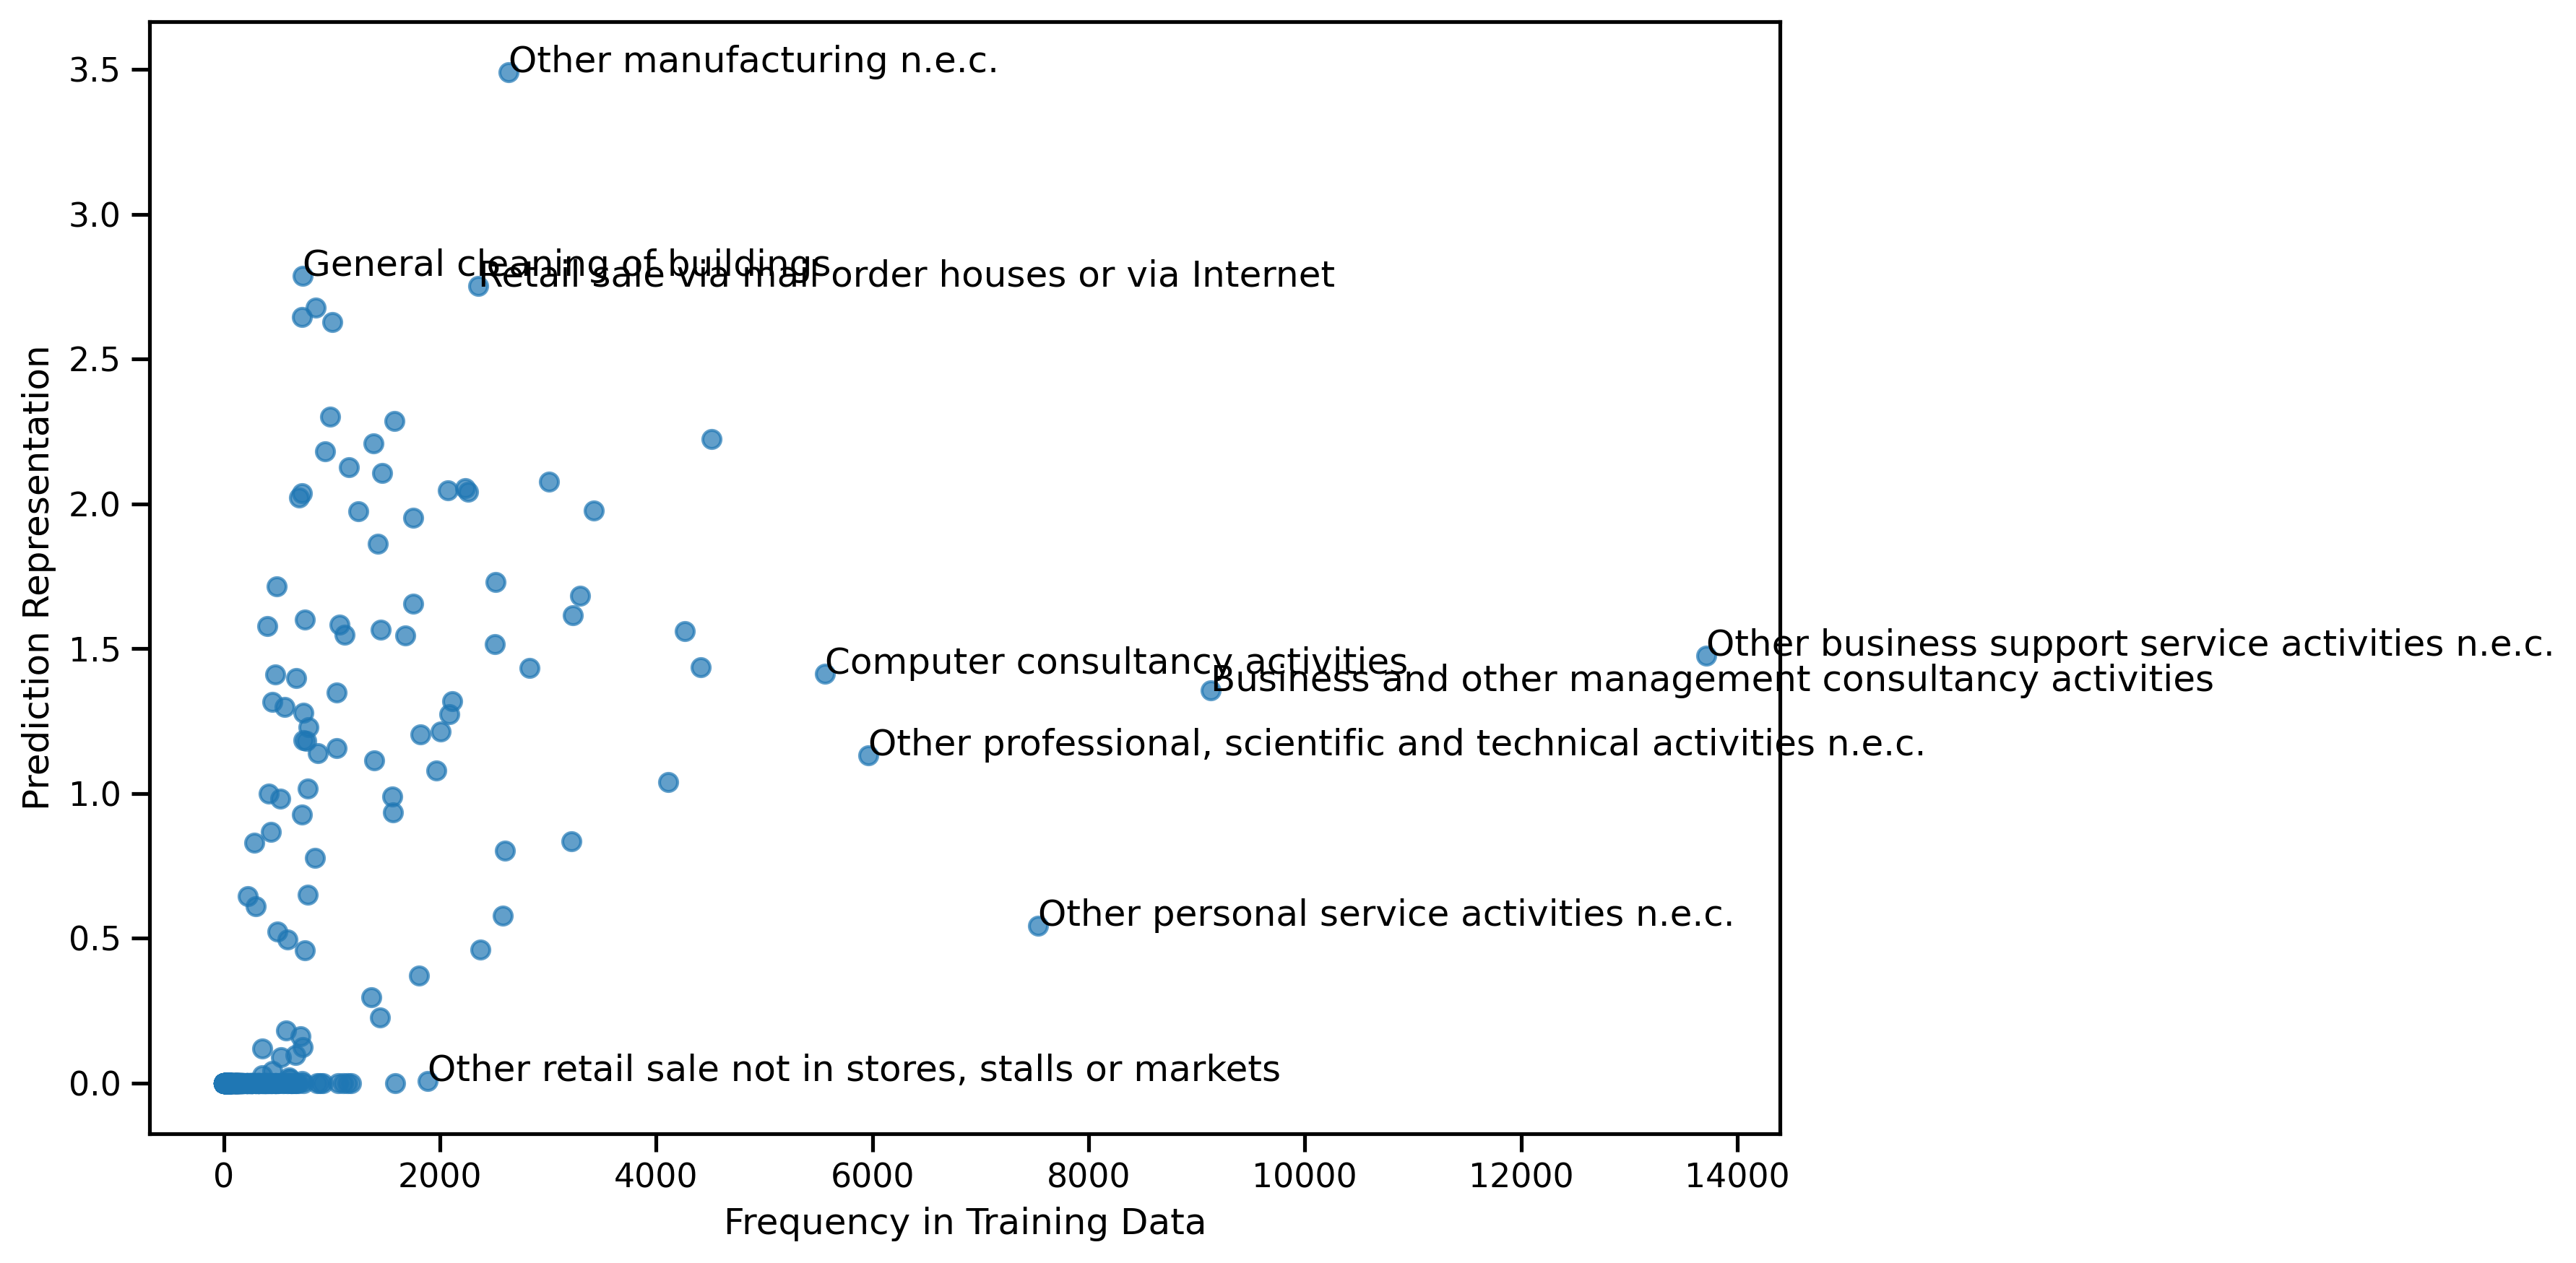
\includegraphics{../../figures/predicted_sic4_representation_vs_training_frequency_scatter.png}

There is also a relationship between the frequency of a code's
appearance in the training data and its average prediction probability
on the test set. The trend in
\{\#fig:mean\_sic4\_prediction\_probability\_vs\_training\_frequency\_scatter\}
shows that although there is a gradual trend with the log of a code's
frequency, there are similarly codes with a low frequency that have a
high average prediction probability.

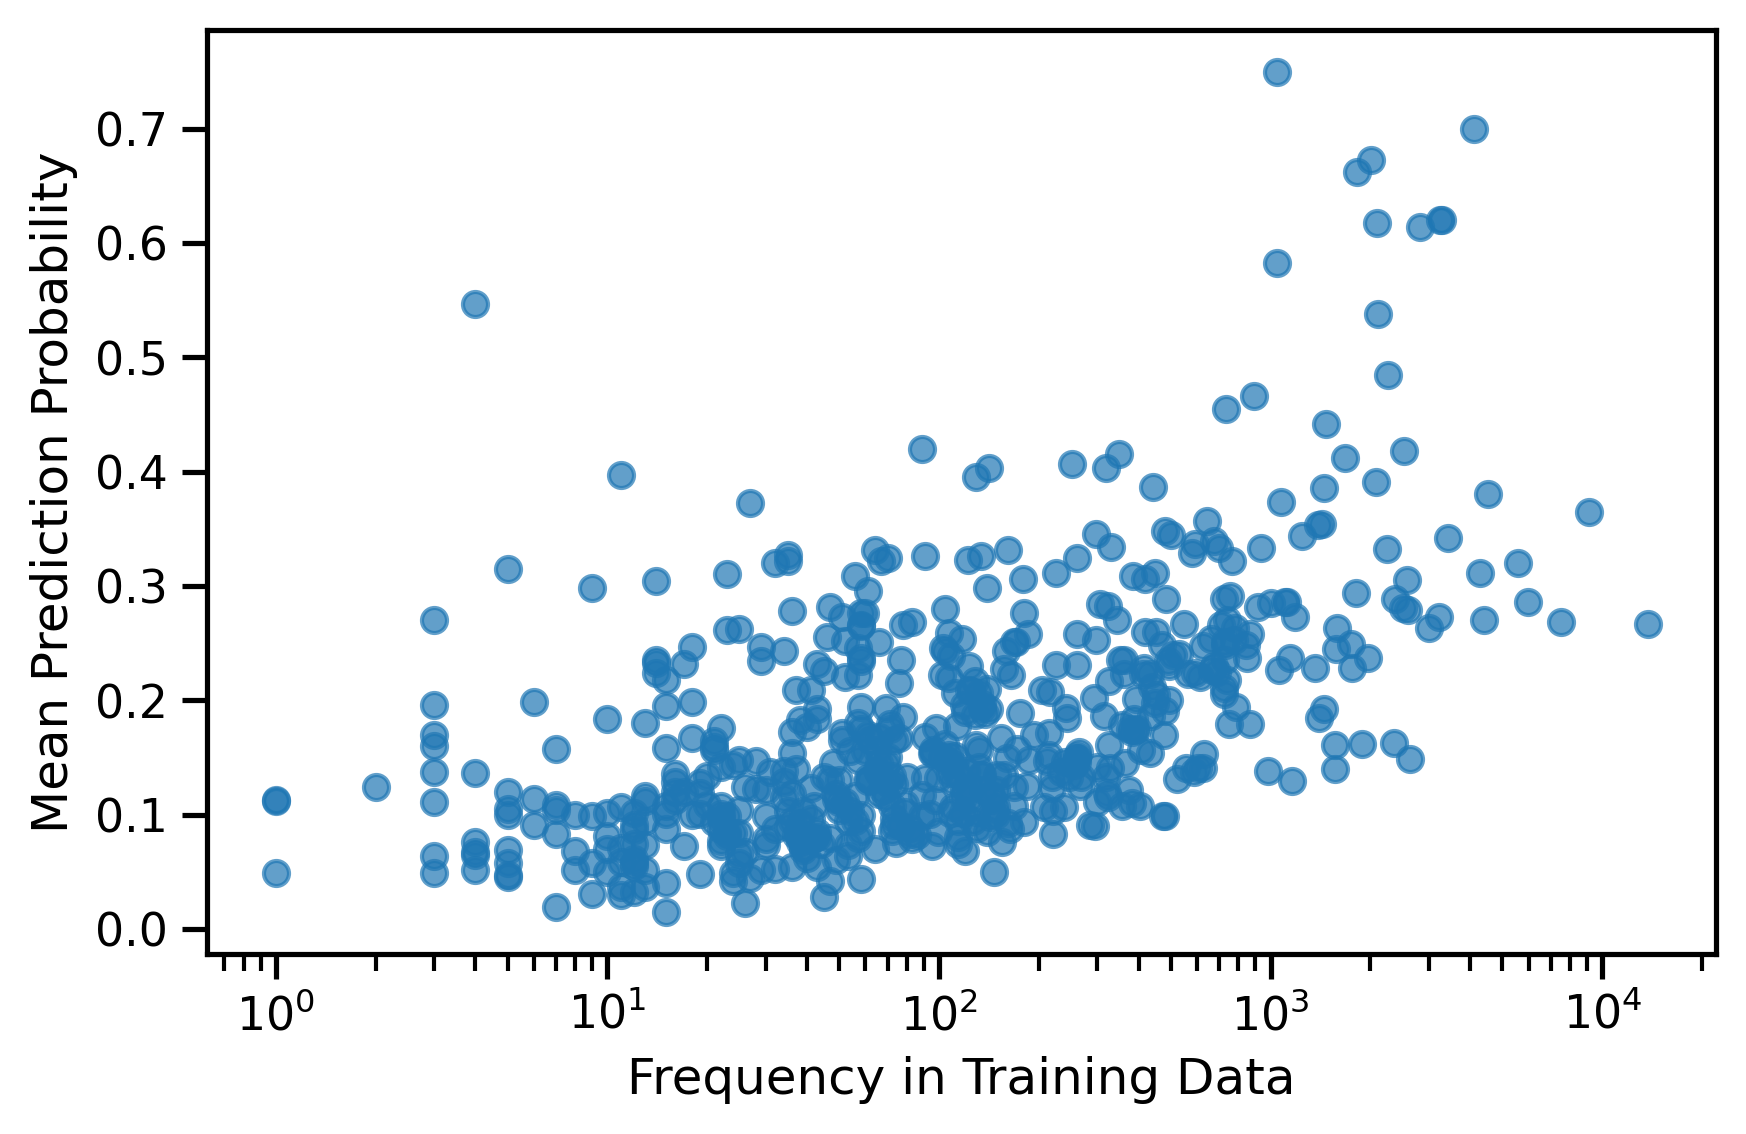
\includegraphics[width=0.5\textwidth,height=\textheight]{../../figures/mean_sic4_prediction_probability_vs_training_frequency_scatter.png}

Finally, we assessed the coherence of the groups of company descriptions
in our predicted categories using the silhouette score. This metric is
normally reserved for assessing the quality of clusters when using an
unsupervised machine learning method, however essentially it measures
the extent to which points in a group are clustered with samples similar
to themselves by looking at the inter-group and intra-group sample
distances. A higher score means that points in a cluster are grouped
tightly and are separated from other clusters. This corresponds to how
similar the descriptions of companies are to each other within a group
of companies with the same predicted 4-digit SIC code and how
semantically separable they are from companies with different predicted
codes.

We encoded the company descriptions as 768 dimensional vectors with a
variant of the BERT transformer pre-trained specifically for semantic
similarity calculations and calculated the silhouette score for each
sample within a specific SIC code before finding the mean. The codes
with the top and bottom average scores are shown in
\{\#fig:predicted\_sic4\_silhouette\_barh\} suggesting that the
descriptions of specific but ubiquitous industries tend to cluster
better in the semantic space created.

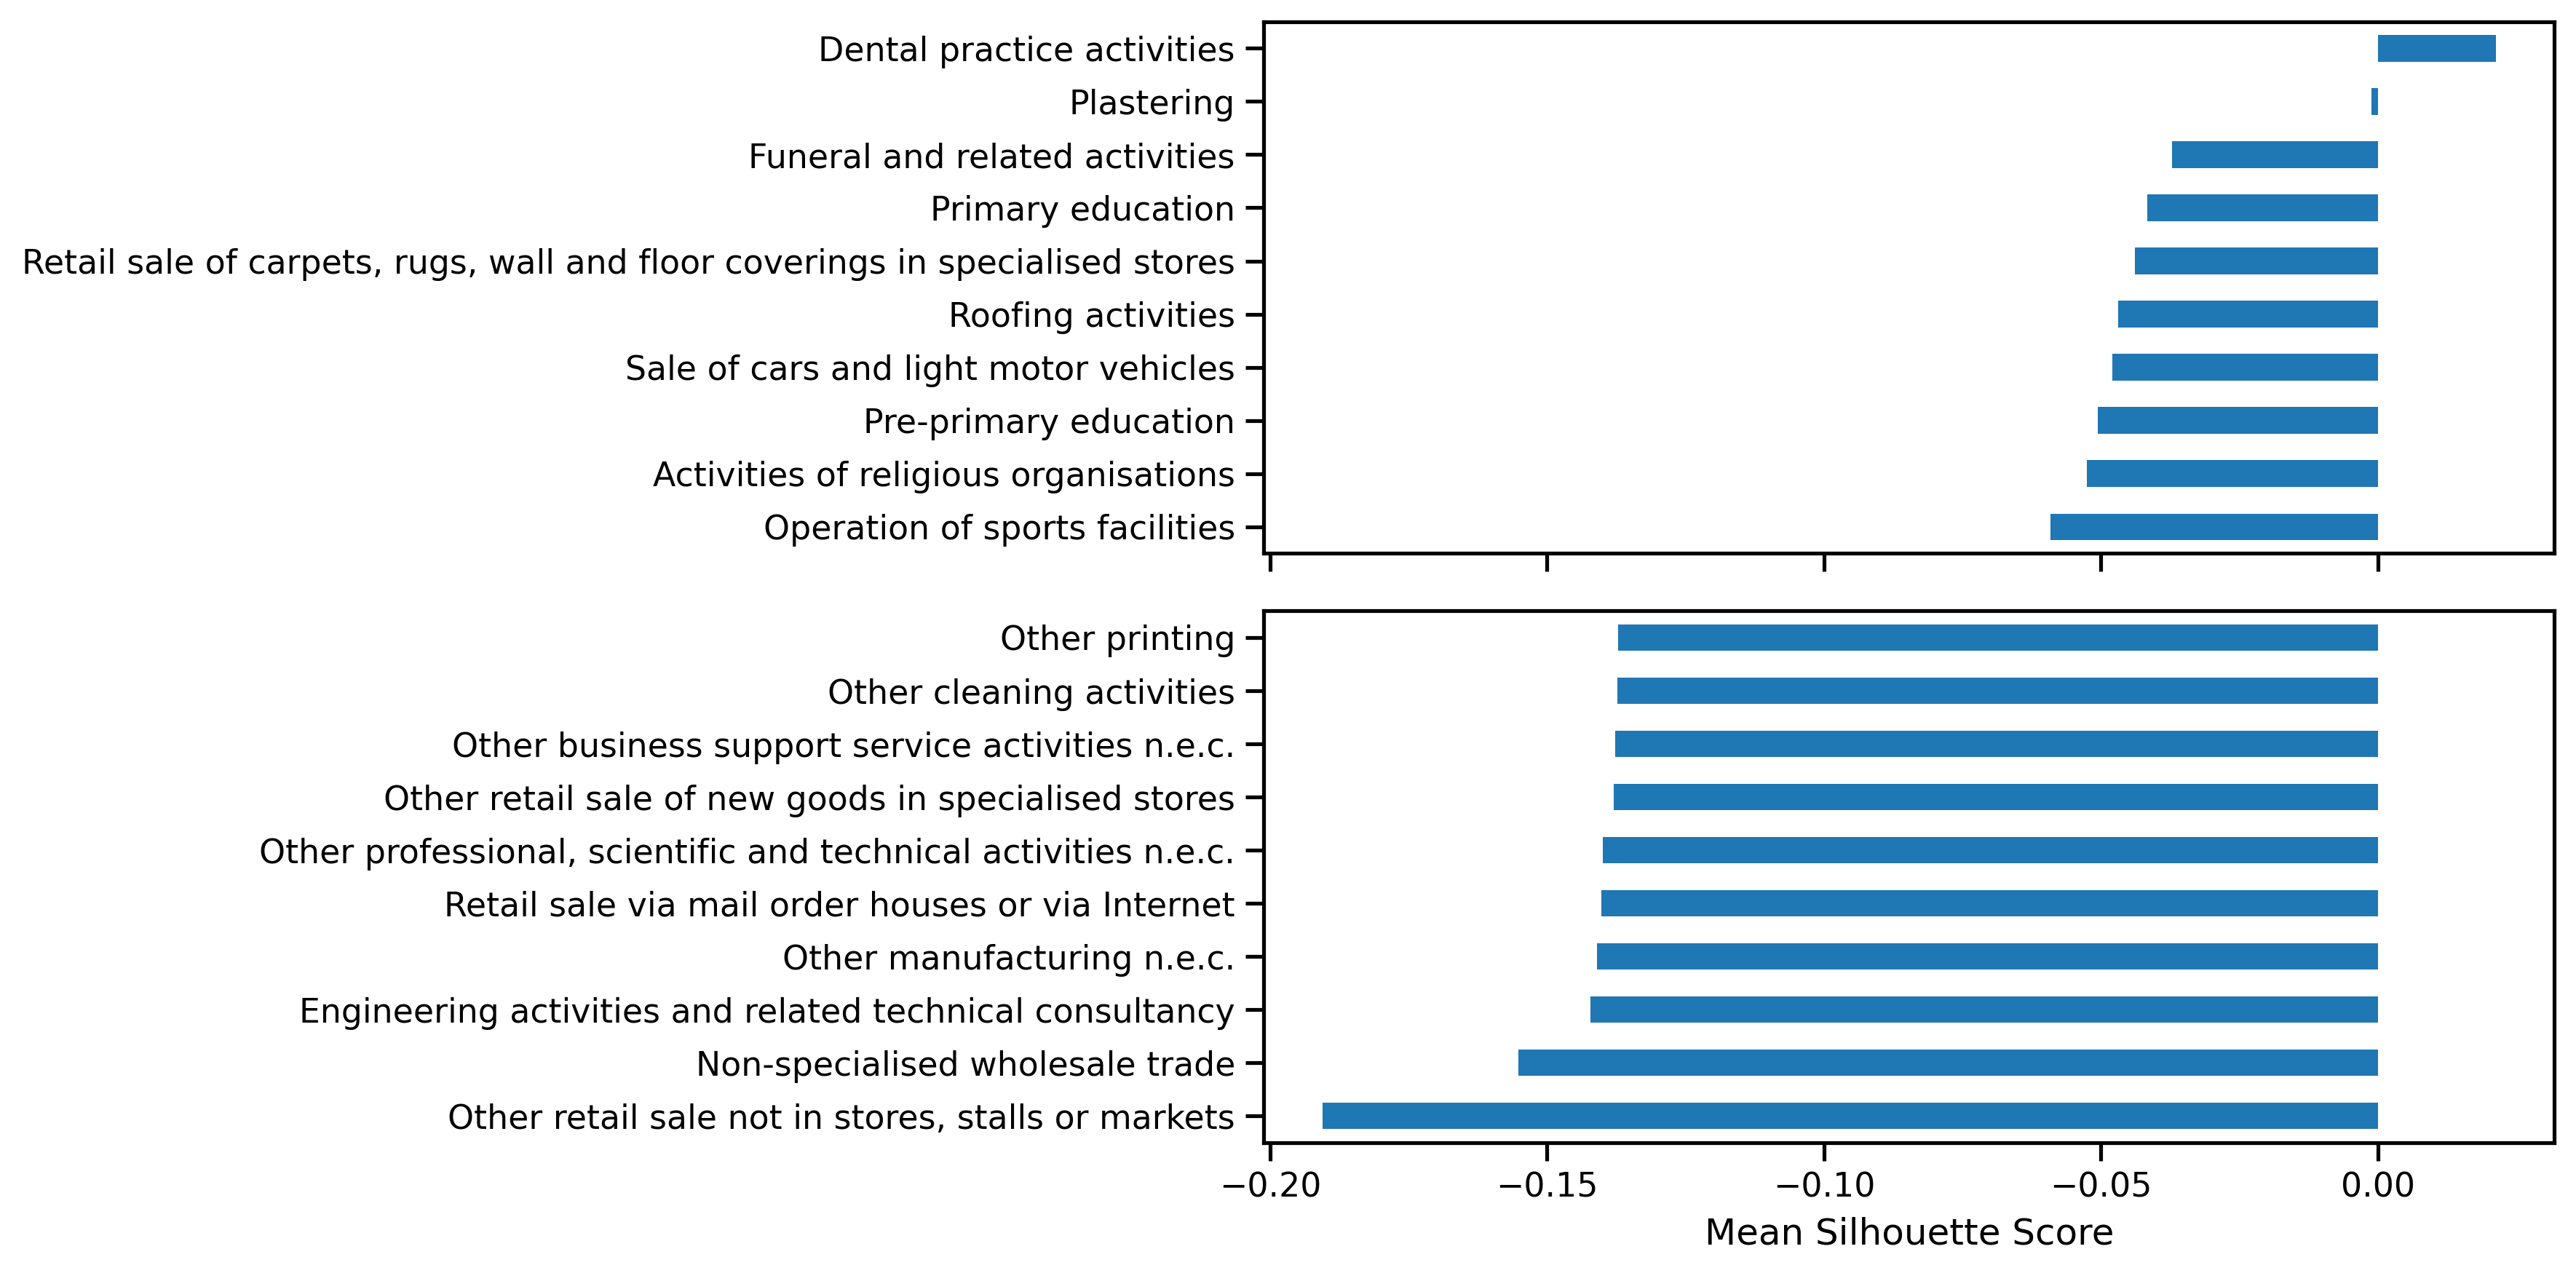
\includegraphics{../../figures/predicted_sic4_silhouette_barh.png}

\hypertarget{next-steps}{%
\subsection{3. Next Steps}\label{next-steps}}

There are two overarching goals from this point. The first is to improve
the classifier through further cleaning of the training data and the
second is to better establish the degree to which the labelling is
limited by the existing SIC taxonomy.

\hypertarget{a.-data-cleaning}{%
\subsubsection{a. Data Cleaning}\label{a.-data-cleaning}}

As mentioned in the previous section, there are SIC codes that bear no
resemblance to the company descriptions they accompany. This may be
because of errors in the Glass AI data or because of the fuzzy matching
process used to link that dataset with Companies House. In either case,
we could improve the training data by removing samples where the 4-digit
SIC code label has a very low semantic similarity with the company
description. This would require establishing a threshold by manual
inspection of the data.

\hypertarget{b.-analysis-of-predictions}{%
\subsubsection{b. Analysis of
Predictions}\label{b.-analysis-of-predictions}}

The predictions produced by the model on a test dataset can be used to
understand the limitations of the existing taxonomy by developing
analyses that take advantage of company descriptions and try to track
down the source of errors in the classifier. There are of course
multiple ways of approaching this. Here we suggest further ways of
measuring the quality of the predicted labels and approaches for
identifying the causes of the model's decisions.

In some cases, one industrial code may not be sufficient to describe a
company's activities. One analysis could be to identify where there are
other possible labels that the model gave a high classification
probability and to see how semantically similar that label is to the top
label predicted. might have predicted. In cases where both labels have a
high probability but a low semantic similarity, it may indicate that
more than one label is required to adequately describe the organisation,
and that possibly the company cuts across diverse industries.

Another could be to further explore the groups of companies in SIC code
groups with a low silhouette score. This would help to identify whether
there are groups of companies that are highly diverse in their
activities but that business owners attempt to group under a single
code.

Additionally we could investigate how far away predicted codes are in
the SIC taxonomy from the labelled codes. This would involve calculating
the distance required to traverse from one code to another across the
taxonomy tree and would tell us how whether the company description
captures activities from a different industrial sector to the one
capture by the labelled code.

Once these further quantitative analyses have been carried out, we could
take a more systematic approach to manually investigating the company
descriptions and their predicted and labelled codes, particularly for
codes or companies that lie at the extremes of the measures described in
this report and for next steps. This would help elucidate the reasons
behind the characteristics of companies that are very readily to
classify and those that are more challenging, as well as the need for
modifications to the taxonomy.

\end{document}
